% Provenance (never printed): see sources/outline_sources.md (Year 3:
% critical-taper theory; fold-and-thrust belts; exhumation and
% thermochronology). Brief: sources/book5/BRIEFS.md, ch. 10. Curves from
% figdata/bachelor-3/fault_bend.py, critical_taper.py and age_elevation.py.
% Exercise and problem values in the Book 5 scratch calculator calc/ch10.py.
\chapter{Cinturones de cabalgamiento y cuñas orogénicas}\label{ch:b3:orogenic-wedges}

Si se empuja una topadora contra arena o nieve húmedas, se acumula una cuña
de material delante de la hoja. Se deforma hasta alcanzar cierta pendiente
en su superficie; a partir de entonces se desliza hacia delante como un todo y crece
con la misma forma, incorporando material nuevo en su pie. Las partes externas de los
cinturones montañosos, desde Taiwán hasta las estribaciones de los Alpes, se comportan igual:
son cuñas de roca raspada de una placa y empujada sobre una base débil, y su pendiente
superficial y el buzamiento de su base indican cuán débil es esa base y cuánta
presión ejercen los fluidos que contiene. Este capítulo construye la geometría de los
cinturones de cabalgamiento, la mecánica de la cuña y los relojes que miden la rapidez
con que sus rocas ascienden hasta la superficie.
% ledger: dsd83:taper

\begin{recall}
Los cabalgamientos, la vergencia y la geometría de los pliegues se tratan en el volumen de primer año, en su capítulo
sobre fallas, pliegues y fábricas; el criterio de Coulomb, la ley de Byerlee, el
esfuerzo efectivo y la razón de presión de poro $\lambda = P/\sigma_v$ en su
capítulo sobre esfuerzo, deformación y reología; la temperatura de cierre y la edad de enfriamiento
en su capítulo sobre métodos de datación radiométrica. El despegue, el
cinturón de pliegues y cabalgamientos, la tectónica de piel fina y de piel gruesa y la
sección equilibrada se tratan en el volumen de segundo año, en su capítulo sobre la anatomía de un
cinturón montañoso; la exhumación y su tasa en su capítulo sobre trayectorias P--T--t. La
construcción de kink y el área en exceso $A = Sh$ de un pliegue sobre un despegue
se tratan en el \cref{ch:b3:structural-analysis}; el \omterm{def:b3:lithosphere-thermal-models:peclet}{número de Péclet térmico} en
el \cref{ch:b3:lithosphere-thermal-models}.
\end{recall}

\section{Geometría de los cabalgamientos}\label{sec:b3:orogenic-wedges:geometry}

Un cabalgamiento no atraviesa una secuencia estratificada a lo largo de un único plano recto.
Sigue una capa débil, una lutita o una evaporita, durante grandes distancias, y luego
asciende abruptamente a través de las capas competentes superiores hasta la siguiente capa débil. La
escalera que dibuja controla los pliegues del bloque superior.

\begin{definition}[Rampa, rellano, dúplex, cabalgamiento fuera de secuencia]\label{def:b3:orogenic-wedges:thrust-geometry}
Un \emph{rellano (de cabalgamiento)}\index{rellano (de cabalgamiento)} es un segmento de cabalgamiento que discurre
paralelo a la estratificación, normalmente en una capa débil; una \emph{rampa
(de cabalgamiento)}\index{rampa (de cabalgamiento)} es un segmento que corta la estratificación,
típicamente de 20 a \ang{30}, que une un rellano inferior con otro superior. Un
\emph{dúplex (de cabalgamiento)}\index{dúplex (de cabalgamiento)} es un apilamiento de láminas limitadas por fallas,
llamadas escamas, encerradas entre un cabalgamiento basal inferior y un cabalgamiento de techo
superior, cada escama limitada por una rampa que une ambos. Los cabalgamientos suelen formarse
en secuencia, cada nuevo cabalgamiento en el bloque inferior del anterior, más cerca del
antepaís; un \emph{cabalgamiento fuera de secuencia}\index{cabalgamiento fuera de secuencia} es
el que se forma o se vuelve a deslizar detrás del frente activo, cortando cabalgamientos más antiguos.
\end{definition}

Al desplazarse el bloque superior sobre una curva de la falla, debe plegarse para mantenerse en
contacto con ella: se forma un sinclinal donde entra en la rampa y un anticlinal
donde sale de ella.

\begin{definition}[Pliegues de flexión de falla, de propagación de falla y de despegue]\label{def:b3:orogenic-wedges:thrust-folds}
Un \emph{pliegue de flexión de falla}\index{pliegue de flexión de falla} es un pliegue del bloque superior
de un cabalgamiento, producido al deslizarse sobre una curva de la falla, una rampa entre
dos rellanos. Un \emph{pliegue de propagación de falla}\index{pliegue de propagación de falla}
crece sobre la punta de un cabalgamiento que aún se propaga hacia arriba: el
acortamiento que la falla ya no transmite se absorbe mediante plegamiento delante de
su punta, lo que da lugar a un flanco frontal empinado o volcado. Un \emph{pliegue de
despegue}\index{pliegue de despegue} crece sobre un rellano sin rampa: el acortamiento
se absorbe por plegamiento y por una capa débil, de sal o lutita, que fluye hacia
su núcleo.
\end{definition}

La figura siguiente construye un \omterm{def:b3:orogenic-wedges:thrust-folds}{pliegue de flexión de falla}. Aquí el bloque superior se desplaza
paralelo al segmento de falla que queda debajo y se pliega según superficies axiales que
bisecan cada curva, un modelo cinemático llamado flujo paralelo a la falla; el clásico
modelo de espesor y longitud de capa constantes da el mismo anticlinal de cima plana
con un flanco frontal más empinado, a costa de una construcción más larga
(que aquí se admite). Ambos modelos están sujetos a la conservación del área.

\begin{omfigure}
\begin{tikzpicture}
\begin{groupplot}[group style={group size=1 by 2, vertical sep=0.9cm},
  width=0.92\linewidth, axis equal image,
  xmin=0, xmax=12, ymin=-0.6, axis lines=none, clip=true,
  title style={font=\small, at={(0.0,1.0)}, anchor=south west}]
% (a) before slip
\nextgroupplot[title={(a) antes del deslizamiento}, ymax=1.75]
\fill[omLithSand!70] (axis cs:0,0) rectangle (axis cs:12,1.6);
\fill[gray!25] (axis cs:0,-0.6) rectangle (axis cs:12,0);
\draw[black!70] (axis cs:0,0.25) -- (axis cs:12,0.25);
\draw[black!70] (axis cs:0,0.5) -- (axis cs:12,0.5);
\draw[black!70] (axis cs:0,0.75) -- (axis cs:12,0.75);
\draw[black!70] (axis cs:0,1.0) -- (axis cs:12,1.0);
\draw[black!70] (axis cs:0,1.3) -- (axis cs:12,1.3);
\draw[black!70] (axis cs:0,1.6) -- (axis cs:12,1.6);
\draw[black!70] (axis cs:0,-0.3) -- (axis cs:12,-0.3);
\addplot[very thick, red!70!black] table[x=x, y=y] {figdata/out/bachelor-3-fault_bend-fault.dat};
\node[font=\scriptsize, fill=omLithSand!70, inner sep=1pt] at (axis cs:2,0.125) {rellano inferior};
\node[font=\scriptsize, fill=omLithSand!70, inner sep=1pt, rotate=30] at (axis cs:4.55,0.62) {rampa};
\node[font=\scriptsize, fill=omLithSand!70, inner sep=1pt] at (axis cs:9,0.875) {rellano superior};
% (b) after a slip of 2.5 units
\nextgroupplot[title={(b) tras el deslizamiento: un pliegue de flexión de falla}, ymax=2.75]
\fill[gray!25] (axis cs:0,-0.6) rectangle (axis cs:12,0) -- cycle;
\addplot[name path=fault, draw=none] table[x=x, y=y] {figdata/out/bachelor-3-fault_bend-fault.dat};
\addplot[name path=top, draw=none] table[x=x, y=y] {figdata/out/bachelor-3-fault_bend-bed6.dat};
\addplot[name path=base, draw=none] coordinates {(0,-0.6) (12,-0.6)};
\addplot[omLithSand!70] fill between[of=fault and top];
\addplot[gray!25] fill between[of=base and fault];
\addplot[black!70] table[x=x, y=y] {figdata/out/bachelor-3-fault_bend-bed1.dat};
\addplot[black!70] table[x=x, y=y] {figdata/out/bachelor-3-fault_bend-bed2.dat};
\addplot[black!70] table[x=x, y=y] {figdata/out/bachelor-3-fault_bend-bed3.dat};
\addplot[black!70] table[x=x, y=y] {figdata/out/bachelor-3-fault_bend-bed4.dat};
\addplot[black!70] table[x=x, y=y] {figdata/out/bachelor-3-fault_bend-bed5.dat};
\addplot[black!70] table[x=x, y=y] {figdata/out/bachelor-3-fault_bend-bed6.dat};
\draw[black!70] (axis cs:4.4330,0.25) -- (axis cs:12,0.25);
\draw[black!70] (axis cs:4.8660,0.5) -- (axis cs:12,0.5);
\draw[black!70] (axis cs:5.2990,0.75) -- (axis cs:12,0.75);
\draw[black!70] (axis cs:0,-0.3) -- (axis cs:12,-0.3);
\addplot[very thick, red!70!black] table[x=x, y=y] {figdata/out/bachelor-3-fault_bend-fault.dat};
\draw[densely dashed, black!60] (axis cs:0,1.6) -- (axis cs:12,1.6);
\node[font=\scriptsize, anchor=south] at (axis cs:2.2,1.65) {regional};
\node[font=\scriptsize, anchor=west] at (axis cs:8.6,2.25) {área en exceso $A = Sr$};
\draw[black!70] (axis cs:8.6,2.25) -- (axis cs:6.6,2.0);
\node[font=\scriptsize, fill=gray!25, inner sep=1pt] at (axis cs:10.6,0.625) {bloque inferior};
\end{groupplot}
\end{tikzpicture}

\par\smallskip{\small (a) Un cabalgamiento con un rellano inferior, una rampa con buzamiento
\ang{30} y un rellano superior, antes del deslizamiento (esquema, con escalas vertical y
horizontal iguales). (b) El mismo tras un desplazamiento de 2.5 veces la altura de la rampa,
calculado mediante flujo paralelo a la falla: un sinclinal al pie de la rampa, un flanco
posterior paralelo a la rampa, una cresta plana elevada en la altura de la rampa $r$, un
flanco anterior y un área en exceso $Sr$ sobre el nivel regional de cada capa situada por encima
del rellano superior.}\label{fig:b3:orogenic-wedges:thrusts}
\end{omfigure}


\begin{proposition}[Área en exceso de un pliegue de flexión de falla]\label{prop:b3:orogenic-wedges:fault-bend-area}
Sea un cabalgamiento que eleva su bloque superior por una rampa de altura $r$ desde un rellano
inferior hasta un rellano superior, con el desplazamiento $S$ sobre el rellano inferior. Para toda capa del
bloque superior situada por encima del rellano superior, el área comprendida entre la capa plegada y su
nivel original es $A = Sr$, la misma para toda capa de este tipo.
\end{proposition}

\begin{proof}
La roca no se crea ni se destruye, y su volumen se conserva. Considérese una sección
paralela al desplazamiento, limitada por dos líneas verticales alejadas por detrás y por delante
de la rampa. A través de la línea trasera, el bloque superior comprendido entre el rellano
inferior y una capa situada a la altura $y_0$ sobre él ha entrado en $S$: el área
$Sy_0$ ha entrado. A través de la línea frontal, la roca comprendida entre el rellano
superior y la misma capa, de espesor $y_0 - r$, ha salido en el desplazamiento del rellano superior,
también $S$ cuando la roca conserva su área: el área $S(y_0 - r)$
ha salido. La diferencia, $Sr$, ha permanecido entre las dos líneas y eleva
la capa por encima de su nivel original.
\end{proof}

El área en exceso de un \omterm{def:b3:orogenic-wedges:thrust-folds}{pliegue de flexión de falla} mide el desplazamiento por la altura de
la rampa, y no por la profundidad hasta el despegue, como ocurriría en un
\omterm{def:b3:orogenic-wedges:thrust-folds}{pliegue de despegue} (véase el \cref{ch:b3:structural-analysis}). Los dos tipos de pliegue
deben distinguirse antes de convertir un área en acortamiento.


Un dúplex (véase la figura siguiente) crece cuando el cabalgamiento, en lugar de llevar su bloque superior
cada vez más lejos por la misma rampa, la abandona y corta una nueva rampa en su bloque inferior,
por delante de la antigua. La lámina comprendida entre la rampa antigua y la nueva se convierte en un
caballo tectónico, elevado por la nueva rampa y apilado bajo el techo; la siguiente rampa
se forma de nuevo por delante. Cada caballo se acorta desde su longitud original hasta la
longitud que ocupa ahora a lo largo del muro, y el acortamiento del dúplex es
la suma de los acortamientos de sus caballos. Los \omterm{def:b3:orogenic-wedges:thrust-geometry}{cabalgamientos fuera de secuencia} alteran este orden: se forman
cuando la cuña situada detrás del frente debe engrosarse, un caso que la mecánica de la
sección siguiente predice.

\begin{omfigure}
\begin{tikzpicture}
\begin{axis}[width=0.92\linewidth, axis equal image, xmin=0, xmax=12, ymin=-0.6, ymax=1.95,
  axis lines=none, clip=true]
\fill[gray!25] (axis cs:0,-0.6) rectangle (axis cs:12,0);
\fill[omLithSand!70] (axis cs:0,0) -- (axis cs:1.0,0) -- (axis cs:2.35,1.15) -- (axis cs:12,1.15) -- (axis cs:12,1.85) -- (axis cs:2.35,1.85) -- (axis cs:1.0,0.7) -- (axis cs:0,0.7) -- cycle;
\draw[black!70] (axis cs:0,0.35) -- (axis cs:1.0,0.35) -- (axis cs:2.35,1.5) -- (axis cs:12,1.5);
\draw[black!70] (axis cs:0,0.7) -- (axis cs:1.0,0.7) -- (axis cs:2.35,1.85) -- (axis cs:12,1.85);
\fill[omLithShale!60] (axis cs:8.2,0) -- (axis cs:12,0) -- (axis cs:12,1.15) -- (axis cs:9.55,1.15) -- cycle;
\draw[black!70] (axis cs:8.646,0.38) -- (axis cs:12,0.38);
\draw[black!70] (axis cs:9.104,0.77) -- (axis cs:12,0.77);
\fill[omLithLime] (axis cs:1.0,0) -- (axis cs:2.80,0) -- (axis cs:4.15,1.15) -- (axis cs:2.35,1.15) -- cycle;
\draw[black!70] (axis cs:1.45,0) -- (axis cs:2.80,1.15);
\draw[black!70] (axis cs:1.90,0) -- (axis cs:3.25,1.15);
\draw[black!70] (axis cs:2.35,0) -- (axis cs:3.70,1.15);
\fill[omLithShale] (axis cs:2.8,0) -- (axis cs:4.60,0) -- (axis cs:5.95,1.15) -- (axis cs:4.15,1.15) -- cycle;
\draw[black!70] (axis cs:3.25,0) -- (axis cs:4.60,1.15);
\draw[black!70] (axis cs:3.70,0) -- (axis cs:5.05,1.15);
\draw[black!70] (axis cs:4.15,0) -- (axis cs:5.50,1.15);
\fill[omLithLime] (axis cs:4.6,0) -- (axis cs:6.40,0) -- (axis cs:7.75,1.15) -- (axis cs:5.95,1.15) -- cycle;
\draw[black!70] (axis cs:5.05,0) -- (axis cs:6.40,1.15);
\draw[black!70] (axis cs:5.50,0) -- (axis cs:6.85,1.15);
\draw[black!70] (axis cs:5.95,0) -- (axis cs:7.30,1.15);
\fill[omLithShale] (axis cs:6.4,0) -- (axis cs:8.20,0) -- (axis cs:9.55,1.15) -- (axis cs:7.75,1.15) -- cycle;
\draw[black!70] (axis cs:6.85,0) -- (axis cs:8.20,1.15);
\draw[black!70] (axis cs:7.30,0) -- (axis cs:8.65,1.15);
\draw[black!70] (axis cs:7.75,0) -- (axis cs:9.10,1.15);
\draw[thick, red!70!black] (axis cs:1.0,0) -- (axis cs:2.35,1.15);
\draw[thick, red!70!black] (axis cs:2.8,0) -- (axis cs:4.15,1.15);
\draw[thick, red!70!black] (axis cs:4.6,0) -- (axis cs:5.95,1.15);
\draw[thick, red!70!black] (axis cs:6.4,0) -- (axis cs:7.75,1.15);
\draw[thick, red!70!black] (axis cs:8.2,0) -- (axis cs:9.55,1.15);
\draw[very thick, red!70!black] (axis cs:0,0) -- (axis cs:12,0);
\draw[very thick, red!70!black] (axis cs:2.35,1.15) -- (axis cs:12,1.15);
\node[font=\scriptsize, anchor=north west] at (axis cs:0.1,-0.04) {cabalgamiento de muro};
\node[font=\scriptsize, anchor=south west] at (axis cs:7.0,1.17) {cabalgamiento de techo};
\node[font=\scriptsize, anchor=north] at (axis cs:5.6,-0.12) {caballo tectónico};
\draw[black!70] (axis cs:5.6,-0.15) -- (axis cs:5.5,0.45);
\draw[->, thick] (axis cs:0.15,0.52) -- (axis cs:0.95,0.52);
\end{axis}
\end{tikzpicture}

\par\smallskip{\small Un dúplex (esquema): cuatro caballos tectónicos (azul y verde) cortados
por rampas entre un cabalgamiento de muro y uno de techo, por delante de ellos el bloque inferior no
cortado aún, la flecha indica el sentido del transporte; la cobertera situada sobre el techo está
plegada sobre el apilamiento.}\label{fig:b3:orogenic-wedges:duplex}
\end{omfigure}


\section{El ahusamiento crítico}\label{sec:b3:orogenic-wedges:taper}

Un cinturón de pliegues y cabalgamientos, en sección transversal, es una cuña: delgada en su frente, donde
el despegue llega a la superficie, y engrosada hacia el interior de la cadena.
Su superficie superior se inclina hacia el antepaís con el ángulo $\alpha$; su
base, el despegue, buza hacia el interior de la cadena con el ángulo $\beta$. El
ahusamiento de la cuña es el ángulo comprendido entre ambas, $\alpha + \beta$.

\begin{definition}[Ahusamiento crítico]\label{def:b3:orogenic-wedges:critical-taper}
El \emph{ahusamiento crítico}\index{ahusamiento crítico} de una cuña empujada desde atrás
sobre una base es el ahusamiento en el que la cuña se encuentra en todas partes al borde de
la rotura, en su interior y a lo largo de su base, bajo compresión horizontal. Una cuña en
su ahusamiento crítico se desliza sobre su base sin deformarse internamente; una
cuña por debajo de él (subcrítica) se deforma y engrosa hasta alcanzarlo; una
cuña por encima de él (supercrítica) se desliza sin deformarse.
\end{definition}
% ledger: dsd83:taper

\begin{omfigure}
\begin{tikzpicture}[>=stealth, x=1cm, y=1cm]
\fill[omLithSand!70] (0,0) -- (10,-1.05) -- (10,1.4) -- cycle;
\fill[gray!25] (0,0) -- (10,-1.05) -- (10,-1.6) -- (-0.8,-1.6) -- (-0.8,0) -- cycle;
\draw[thick] (-0.8,0) -- (0,0) -- (10,1.4);
\draw[very thick, red!70!black] (0,0) -- (10,-1.05);
\fill[gray!60] (10,-1.6) rectangle (10.6,1.9);
\node[font=\scriptsize, rotate=90] at (10.3,0.15) {tope};
\draw[dashed] (0,0) -- (2.6,0);
\draw (2.2,0) arc[start angle=0, end angle=8, radius=2.2];
\node[font=\small] at (2.45,0.2) {$\alpha$};
\draw (2.2,0) arc[start angle=0, end angle=-6, radius=2.2];
\node[font=\small] at (2.45,-0.2) {$\beta$};
% slice
\draw[thick, omDef] (5.5,-0.5775) -- (5.5,0.77);
\draw[thick, omDef] (6.5,-0.6825) -- (6.5,0.91);
\draw[->, thick, omDef] (4.5,0.05) -- (5.45,0.05);
\node[font=\scriptsize, anchor=east] at (4.5,0.05) {$F(x)$};
\draw[<-, thick, omDef] (6.55,0.1) -- (7.6,0.1);
\node[font=\scriptsize, anchor=west] at (7.6,0.1) {$F(x + \mathrm dx)$};
\draw[->, thick, omProp] (6.0,-0.63) -- (6.75,-0.71);
\node[font=\scriptsize, anchor=north] at (6.4,-0.75) {$\tau_b$};
\draw[->, thick, omProp] (6.0,-0.63) -- (6.1,0.0);
\node[font=\scriptsize, anchor=east] at (6.02,-0.22) {$\sigma_n$};
\node[font=\scriptsize] at (6.0,1.2) {rebanada $\mathrm dx$};
\draw[->, thick] (1.8,-1.25) -- (0.6,-1.25);
\node[font=\scriptsize, anchor=west] at (1.85,-1.25) {transporte};
\node[font=\scriptsize, anchor=west] at (0.2,-0.42) {despegue};
\node[font=\scriptsize] at (8.9,-0.45) {cuña};
\draw[->] (0.1,0.5) -- (0.4,0.5); \node[font=\scriptsize, anchor=east] at (0.1,0.5) {$x$};
\end{tikzpicture}

\par\smallskip{\small Una cuña de pendiente superficial $\alpha$ apoyada sobre un
despegue de buzamiento $\beta$ y empujada desde atrás; $x$ se mide desde el
pie hacia el hinterland. En un corte vertical, el empuje $F(x + \mathrm dx)$
desde atrás supera al empuje $F(x)$ desde el frente en lo que retiene la base:
su fricción $\tau_b$ y la parte horizontal de su esfuerzo normal $\sigma_n$,
que se inclina hacia el hinterland sobre una base que buza en ese sentido (esquemático,
ángulos exagerados).}\label{fig:b3:orogenic-wedges:wedge}
\end{omfigure}

\begin{theorem}[Ecuación del ahusamiento crítico]\label{thm:b3:orogenic-wedges:critical-taper}
Considérese una cuña subaérea de densidad uniforme $\rho$ formada por material de Coulomb sin cohesión
de fricción interna $\mu = \tan\phi$, con la
razón de presión de poros $\lambda$, sobre una base de fricción $\mu_b$ y razón de
presión de poros $\lambda_b$. Si $\alpha$ y $\beta$ son pequeños y $\sigma_1$ es horizontal,
la \emph{ecuación del ahusamiento crítico}\index{ecuación del ahusamiento crítico} es
\[
  \alpha + \beta = \frac{\beta + \mu_b(1 - \lambda_b)}{1 + K(1 - \lambda)},
  \qquad K = \frac{2\sin\phi}{1 - \sin\phi},
\]
con los ángulos en radianes.
\end{theorem}

\begin{proof}
Sea $z$ la profundidad bajo la superficie. Con pendientes pequeñas, el esfuerzo vertical
es el peso de la roca suprayacente, $\sigma_{zz} = \rho g z$, y la presión
de poros es $\lambda\rho g z$, de modo que el esfuerzo vertical efectivo es
$(1 - \lambda)\rho g z$. En todas partes, en rotura y con $\sigma_1$ horizontal,
el criterio de Coulomb para un material sin cohesión da la razón de los
esfuerzos principales efectivos $\sigma'_1/\sigma'_3 = (1 + \sin\phi)/(1 -
\sin\phi) = 1 + K$, por tanto, el esfuerzo horizontal total
\[
  \sigma_{xx} = (1 + K)(1 - \lambda)\rho g z + \lambda\rho g z
  = \bigl(1 + K(1 - \lambda)\bigr)\rho g z .
\]
A la distancia $x$ del pie, la cuña tiene el espesor $H = (\alpha +
\beta)x$, y la fuerza horizontal por unidad de longitud del cinturón sobre una
sección vertical es $F = \int_0^H \sigma_{xx}\,\mathrm dz = \bigl(1 + K(1 -
\lambda)\bigr)\rho g H^2/2$. En la rebanada comprendida entre $x$ y $x + \mathrm dx$
(véase la figura anterior), la superficie no soporta esfuerzo y el empuje desde atrás
supera al empuje del frente en $(\mathrm dF/\mathrm dx)\,\mathrm dx$.
La base retiene la rebanada de dos maneras: la fricción $\mu_b(1 -
\lambda_b)\rho g H$ por unidad de longitud, y su esfuerzo normal $\rho g H$, que
es perpendicular a una base que buza $\beta$ hacia el hinterland y por eso
se inclina en ese sentido un ángulo $\beta$, lo que da la parte horizontal $\beta\rho g H$.
El equilibrio de la rebanada exige
\[
  \bigl(1 + K(1 - \lambda)\bigr)\rho g H(\alpha + \beta)
  = \bigl(\beta + \mu_b(1 - \lambda_b)\bigr)\rho g H ,
\]
que es la ecuación. Como $H$ se cancela, una cuña en rotura conserva el mismo
ahusamiento al crecer.
\end{proof}

La ecuación indica, en primer lugar, que el ahusamiento viene fijado por la razón entre la resistencia
de la base, en el numerador, y la resistencia de la cuña, en el
denominador: una base débil da una cuña delgada, y una base resistente una gruesa.
En segundo lugar, la pendiente superficial disminuye a medida que la base buza con mayor inclinación. En tercer lugar, la presión de fluidos
reduce el ahusamiento: al aumentar $\lambda = \lambda_b$ se resta más a la
resistencia de la base, en proporción, que a la de la cuña.
La figura siguiente muestra la pendiente superficial crítica para los coeficientes de fricción
ajustados en el oeste de Taiwán. Los puntos situados bajo cada línea corresponden a cuñas subcríticas, que engrosan;
los situados encima, a cuñas supercríticas, que se deslizan.
% ledger: dsd83:taper

\begin{omfigure}
\begin{tikzpicture}
\begin{axis}[omrecord, width=0.8\linewidth, height=0.5\linewidth,
  xlabel={buzamiento basal $\beta$ (\unit{\degree})}, ylabel={pendiente superficial $\alpha$ (\unit{\degree})},
  xmin=0, xmax=15, ymin=0, ymax=12, legend style={font=\scriptsize, at={(0.98,0.98)},
  anchor=north east, legend cell align=left}]
% computed in figdata/bachelor-3/critical_taper.py
\addplot[name path=t3, draw=none, forget plot] table[x=beta, y=t3] {figdata/out/bachelor-3-critical_taper-bands.dat};
\addplot[name path=t4, draw=none, forget plot] table[x=beta, y=t4] {figdata/out/bachelor-3-critical_taper-bands.dat};
\addplot[name path=t12, draw=none, forget plot] table[x=beta, y=t12] {figdata/out/bachelor-3-critical_taper-bands.dat};
\addplot[name path=t13, draw=none, forget plot] table[x=beta, y=t13] {figdata/out/bachelor-3-critical_taper-bands.dat};
\addplot[omLithEvap, area legend] fill between[of=t3 and t4];
\addlegendentry{ahusamiento 3--\ang{4} (Jura)}
\addplot[omLithLime, area legend] fill between[of=t12 and t13];
\addlegendentry{ahusamiento 12--\ang{13}}
\addplot[omDef, thick] table[x=beta, y=a040] {figdata/out/bachelor-3-critical_taper-curves.dat};
\addlegendentry{$\lambda = 0.4$}
\addplot[red!70!black, thick, densely dashed] table[x=beta, y=a070] {figdata/out/bachelor-3-critical_taper-curves.dat};
\addlegendentry{$\lambda = 0.7$}
\addplot[black, thick, densely dotted] table[x=beta, y=a090] {figdata/out/bachelor-3-critical_taper-curves.dat};
\addlegendentry{$\lambda = 0.9$}
\node[font=\scriptsize] at (axis cs:2.2,1.1) {subcrítico};
\node[font=\scriptsize] at (axis cs:1.6,8.6) {supercrítico};
\end{axis}
\end{tikzpicture}

\par\smallskip{\small Pendiente superficial crítica frente al buzamiento basal para los
coeficientes de fricción de Taiwán occidental, $\mu = 1.03$ en el interior y $\mu_b =
0.85$ en la base, para tres razones de presión de poro $\lambda = \lambda_b$;
«subcrítico» y «supercrítico» se refieren a la línea de $\lambda = 0.7$.
Las franjas sombreadas son los ahusamientos de la cuña de cabalgamientos del Jura, de 3 a \ang{4}, y de la
cuña situada al sur de ella, de 12 a \ang{13}.}\label{fig:b3:orogenic-wedges:taper}
\end{omfigure}
% ledger: dsd83:taper, deville21:jura

Una cuña no es un objeto estático: se le añade material y se le quita material,
y cada cambio la desplaza de su \omterm{def:b3:orogenic-wedges:critical-taper}{ahusamiento crítico}.

\begin{definition}[Acreción frontal, subplacado tectónico]\label{def:b3:orogenic-wedges:accretion}
La \emph{acreción frontal}\index{acreción frontal} es la adición de material
a una cuña en su pie, a medida que el despegue se propaga hacia los
sedimentos no deformados del antepaís y se corta una nueva lámina de cabalgamiento. El \emph{subplacado
tectónico}\index{subplacado tectónico} es la adición de material a la
base de la cuña, detrás de su pie, a medida que las láminas de la placa inferior se
despegan y se apilan debajo de ella, a menudo en forma de dúplex.
\end{definition}

La \omterm{def:b3:orogenic-wedges:accretion}{acreción frontal} alarga la cuña a ahusamiento constante. El subplacado engrosa su parte posterior y
empina su superficie: la cuña se vuelve supercrítica allí y puede extenderse por falla normal hasta que
el ahusamiento vuelva a descender. La erosión
hace lo contrario: rebaja la pendiente superficial, y la cuña se vuelve
subcrítica, y se engrosa por \omterm{def:b3:orogenic-wedges:thrust-geometry}{cabalgamientos fuera de secuencia} detrás del frente.
Erosión y deformación están, por tanto, acopladas: una cuña erosionada deprisa conserva
su ahusamiento desplazando la roca hacia arriba más deprisa, y las rocas que lleva a la superficie
son más jóvenes en el sentido de la siguiente sección.

\begin{inthelab}[Modelos en caja de arena]
\begin{minipage}[t]{0.55\linewidth}\vspace{0pt}
En un modelo analógico en caja de arena, se disponen capas de arena seca de distintos colores
dispuestas horizontalmente en una caja alargada de paredes de vidrio. Un motor empuja lentamente una pared vertical contra ellas,
o tira de una lámina por debajo de ellas; una cámara junto al vidrio fotografía la sección a
intervalos regulares. La arena falla a lo largo de cabalgamientos, forma una cuña que mantiene un
ahusamiento constante, y desarrolla rampas, dúplex y retrocabalgamientos como los de los
cinturones reales. Una capa de bolitas de vidrio o de masilla de silicona bajo la arena desempeña
el papel de un despegue débil, y la cuña entonces crece más delgada y más ancha.
Davis, Suppe y Dahlen hallaron que sus experimentos con arena seca concordaban con la
teoría del \omterm{def:b3:orogenic-wedges:critical-taper}{ahusamiento crítico}. La correlación de las fotografías sucesivas proporciona el
campo de desplazamientos en el interior del modelo.
\end{minipage}\hfill
\begin{minipage}[t]{0.42\linewidth}\vspace{0pt}
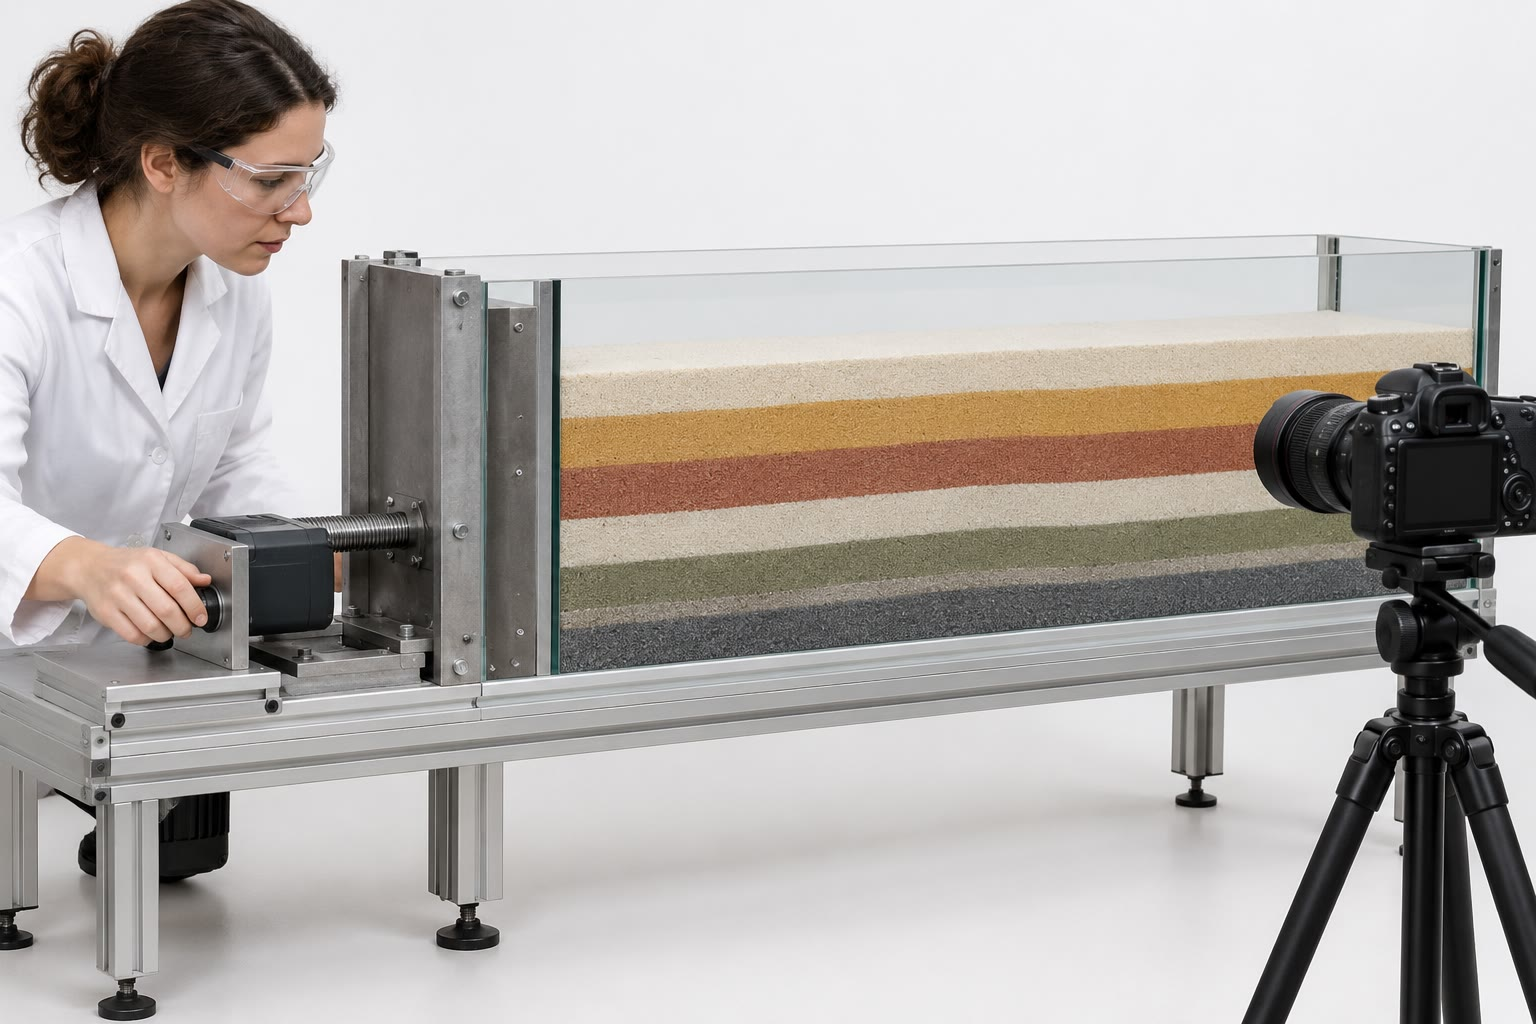
\includegraphics[width=\linewidth]{images/book5/ai/b3-sandbox-lab.jpg}

{\scriptsize Modelo en caja de arena antes del acortamiento: capas de arena de colores en una
caja de paredes de vidrio, una pared accionada por motor a la izquierda, una cámara sobre un trípode
(Ilustración generada por IA.)}
\end{minipage}
\end{inthelab}
% ledger: dsd83:taper

\section{Cuñas reales}\label{sec:b3:orogenic-wedges:real}

En el cinturón activo de pliegues y cabalgamientos del oeste de Taiwán, la pendiente superficial, el
buzamiento del despegue y las presiones de poro son conocidos, a partir de la topografía,
secciones sísmicas y pozos. Davis, Suppe y Dahlen los emplearon para resolver la
\omterm{thm:b3:orogenic-wedges:critical-taper}{ecuación del ahusamiento crítico} para la resistencia de la cuña y hallaron $\mu = 1.03$
en el interior y $\mu_b = 0.85$ en la base: la fricción de Byerlee en la base, y una
cuña más resistente que sus propias fallas, porque no todas están orientadas para
deslizar con facilidad. Con estos dos coeficientes convirtieron los ahusamientos observados de otras
cuñas activas, en tierra y bajo el mar, en razones de presión de poro, y las hallaron
por encima de la hidrostática en todas partes, de acuerdo con las perforaciones. También hallaron
dónde deja de funcionar la teoría: el ahusamiento cae bruscamente cuando las cuñas crecen más gruesas
que unos \qty{15}{km}, profundidad a la que las rocas ricas en cuarzo se vuelven plásticas
para las geotermas habituales, y la base ya no obedece una ley de fricción.
% ledger: dsd83:taper

En el frente de los Alpes occidentales, el Jura es una cuña de cabalgamientos con un
ángulo estrecho de solo 3 a \ang{4}. Su despegue se encuentra sobre todo en capas con halita
de edad triásica, y los fluidos allí no están sobrepresionados: la debilidad de la sal por sí sola
explica el ahusamiento estrecho. Al sur del Jura, donde las
capas triásicas no contienen halita, el mismo frente tiene un ahusamiento de 12 a
\ang{13}, con apilamientos de láminas de cabalgamiento, aunque las presiones de fluido medidas
allí son altas. En los Alpes centrales, el análisis de \omterm{def:b3:orogenic-wedges:critical-taper}{ahusamiento crítico} de la pendiente
superficial da una resistencia basal $\mu_b(1 - \lambda_b)$ (con un pequeño término de
cohesión) inferior a 0.1, e incluso 0.05 en evaporitas y lutitas cerca del frente,
que aumenta hacia el interior de la cadena, con razones de presión de poro superiores a 0.54. La
base de una cuña suele ser mucho más débil de lo que haría la ley de Byerlee, por su
tipo de roca y por sus fluidos.
% ledger: deville21:jura, vonhagke14:alps

\section{Flujo a través de una cuña}\label{sec:b3:orogenic-wedges:flux}

Una cuña en su \omterm{def:b3:orogenic-wedges:critical-taper}{ahusamiento crítico} crece por acreción, a forma constante: su longitud
y su altura aumentan a la vez. La erosión retira roca de su superficie. Cuando ambos
se equilibran, la cuña conserva su tamaño y la roca la atraviesa.

\begin{proposition}[Balance de flujo en estado estacionario]\label{prop:b3:orogenic-wedges:flux}
Una cuña de anchura $W$ a lo largo de la dirección de transporte recibe, por unidad de longitud
del cinturón, el flujo de acreción $F_a = v h$, donde $v$ es la tasa de
convergencia y $h$ el espesor de la capa entrante sobre el despegue. Pierde
el flujo erosivo $F_e = \bar e W$, donde $\bar e$ es la tasa media de
erosión sobre su superficie. Su área de sección varía al ritmo $F_a -
F_e$; en estado estacionario, $\bar e = vh/W$.
\end{proposition}

\begin{proof}
En la unidad de tiempo, una longitud $v$ de la capa entrante, de espesor $h$, pasa
a la cuña a través de su pie, y el espesor $e(x)$ se retira en cada
punto de su superficie; el área se conserva, de modo que el área de la sección
varía en $vh - \int_0^W e\,\mathrm dx = F_a - F_e$. En estado estacionario la
variación es nula.
\end{proof}

Con $v = \qty{10}{mm/yr}$, $h = \qty{4}{km}$ y $W = \qty{60}{km}$, la
tasa de erosión necesaria para el estado estacionario es $\qty{0.67}{mm/yr}$. La exhumación en el
sentido del volumen de segundo año es la retirada de la roca situada encima de una roca dada:
en estado estacionario, las rocas llegan a la superficie a la tasa con que la erosión
la rebaja, y la cuña las eleva desde profundidades donde estaban calientes. Medir la rapidez
requiere un reloj que arranque a una temperatura conocida.

\section{Termocronología}\label{sec:b3:orogenic-wedges:thermochronology}

\begin{definition}[Termocronología, termocronómetro]\label{def:b3:orogenic-wedges:thermochronology}
La \emph{termocronología}\index{termocronología} es el uso de
edades de enfriamiento radiométricas para datar el momento en que una roca pasó por una temperatura dada,
y reconstruir así su historia térmica. Un
\emph{termocronómetro}\index{termocronómetro} es la pareja formada por un mineral y
un método de datación junto con su temperatura de cierre: por ejemplo, el apatito con el
método (U--Th)/He, o el circón con trazas de fisión.
\end{definition}

La tabla siguiente ordena los principales \omterm{def:b3:orogenic-wedges:thermochronology}{termocronómetros} por su temperatura de cierre;
las profundidades suponen una temperatura superficial media de \qty{10}{\celsius} y un
gradiente uniforme de \qty{30}{\celsius/km}. Una roca que se enfría al ser
exhumada los atraviesa uno tras otro, y sus edades crecen desde los métodos de baja
temperatura hasta los de alta temperatura. La física de las trazas de fisión y de la
difusión de helio, que fija estas temperaturas, se expone en
el \cref{ch:b3:advanced-geochronology}.
\begin{center}
\small
% ledger: sueoka19:closure
\begin{tabular}{lcc}
\hline
\omterm{def:b3:orogenic-wedges:thermochronology}{termocronómetro} & temperatura de cierre (\unit{\celsius}) & profundidad (\unit{km}) \\
\hline
apatito (U--Th)/He & 50--80 & 1.3--2.3 \\
apatito, trazas de fisión & 90--120 & 2.7--3.7 \\
circón (U--Th)/He & 160--200 & 5.0--6.3 \\
circón, trazas de fisión & unos 280 & 9 \\
\textsuperscript{40}Ar/\textsuperscript{39}Ar en biotita & 350--400 & 11--13 \\
\textsuperscript{40}Ar/\textsuperscript{39}Ar en moscovita & unos 425 & 14 \\
U--Pb en circón & por encima de 900 & --- \\
\hline
\end{tabular}
\end{center}

Estas profundidades son solo una primera aproximación, porque la erosión modifica la geoterma.

\begin{proposition}[Geoterma en estado estacionario con erosión]\label{prop:b3:orogenic-wedges:geotherm}
Sea una roca que asciende a velocidad constante $v$ a través de una capa de espesor $L$ cuya
superficie ($z = 0$) se mantiene a $T_s$ y la base a $T_L$, sin
producción de calor. La temperatura estacionaria es
\[
  T(z) = T_s + (T_L - T_s)\,\frac{1 - e^{-\mathrm{Pe}\,z/L}}{1 - e^{-\mathrm{Pe}}},
  \qquad \mathrm{Pe} = \frac{vL}{\kappa},
\]
y el gradiente en la superficie es $\mathrm{Pe}/(1 - e^{-\mathrm{Pe}})$ veces
el gradiente conductivo $(T_L - T_s)/L$.
\end{proposition}

\begin{proof}
Una partícula de roca a la profundidad $z$ se mueve hacia arriba, hacia valores menores de $z$: la
temperatura que transporta cambia como $\partial T/\partial t - v\,\partial
T/\partial z$, y la ecuación de difusión queda $\partial T/\partial t - v
T' = \kappa T''$. En estado estacionario, $T'' = -(v/\kappa)T'$, luego $T' = C
e^{-vz/\kappa}$ y $T = T_s + C(\kappa/v)(1 - e^{-vz/\kappa})$, que cumple
$T(0) = T_s$. Imponer $T(L) = T_L$ fija $C$ y da la fórmula. En $z =
0$, $T' = (T_L - T_s)(\mathrm{Pe}/L)/(1 - e^{-\mathrm{Pe}})$.
\end{proof}

Para $\mathrm{Pe} \ll 1$ el factor tiende a 1: domina la conducción y la
geoterma sigue siendo recta. Para $v = \qty{1}{mm/yr}$ a lo largo de \qty{30}{km}, con
$\kappa = \qty{e-6}{m^2/s}$, $\mathrm{Pe} = 0.95$ y el gradiente superficial
sube de 30 a \qty{46}{\celsius/km}: las isotermas se apiñan hacia la
superficie y cada \omterm{def:b3:orogenic-wedges:thermochronology}{termocronómetro} cierra a menor profundidad.
% ledger: england:kelvin, earle:settings

\begin{definition}[Relación edad--altitud]\label{def:b3:orogenic-wedges:age-elevation}
La \emph{relación edad--altitud}\index{relación edad--altitud} de un
\omterm{def:b3:orogenic-wedges:thermochronology}{termocronómetro} es la gráfica de las edades de enfriamiento de muestras recogidas en un
intervalo de altitudes, normalmente a lo largo de una ladera empinada o de un perfil vertical,
frente a sus altitudes.
\end{definition}

\begin{proposition}[Pendiente de la relación edad--altitud]\label{prop:b3:orogenic-wedges:age-elevation}
Sean rocas que ascienden verticalmente a velocidad constante $v$ bajo una
topografía estacionaria, y sea la isoterma de cierre situada a la altitud $e(x) = e_0 +
f\,h(x)$, donde $h(x)$ es la altitud de la superficie y $0 \le f < 1$. Una muestra
recogida en la superficie a la altitud $h$ tiene la edad $t = (h - e)/v$,
y la \omterm{def:b3:orogenic-wedges:age-elevation}{relación edad--altitud} es una recta de pendiente
\[
  \frac{\mathrm dh}{\mathrm dt} = \frac{v}{1 - f}.
\]
Con una isoterma plana, $f = 0$ y la pendiente es la tasa de exhumación.
\end{proposition}

\begin{proof}
La roca que hoy está en la superficie en $x$ atravesó la isoterma de cierre situada justo
debajo, a la altitud $e(x)$, y desde entonces ha ascendido $h - e$ a la velocidad $v$:
$t = (h - e_0 - fh)/v = ((1 - f)h - e_0)/v$. Por tanto $\mathrm dt/\mathrm dh =
(1 - f)/v$.
\end{proof}

\begin{omfigure}
\begin{tikzpicture}
\begin{groupplot}[group style={group size=2 by 1, horizontal sep=1.7cm},
  omrecord, width=0.47\linewidth, height=0.45\linewidth, title style={font=\small},
  legend style={font=\scriptsize, legend cell align=left}]
\nextgroupplot[title={(a) edad--altitud}, xlabel={edad de (U--Th)/He en apatito (\unit{Myr})},
  ylabel={altitud sobre la media (\unit{km})}, xmode=log, xmin=0.1, xmax=10,
  log ticks with fixed point, xtick={0.1,0.2,0.5,1,2,5,10}, ymin=-1, ymax=1]
% computed in figdata/bachelor-3/age_elevation.py
\addplot[black, thick, densely dotted] table[x=a30, y=h] {figdata/out/bachelor-3-age_elevation-ages.dat};
\addplot[red!70!black, thick, densely dashed] table[x=a10, y=h] {figdata/out/bachelor-3-age_elevation-ages.dat};
\addplot[omDef, thick] table[x=a03, y=h] {figdata/out/bachelor-3-age_elevation-ages.dat};
\nextgroupplot[title={(b) la isoterma de cierre}, xlabel={distancia (\unit{km})},
  ylabel={altitud sobre la media (\unit{km})}, xmin=0, xmax=40, ymin=-3.3, ymax=1.2,
  legend style={at={(0.5,0.03)}, anchor=south, legend columns=2}]
\addplot[black!70, very thick] table[x=x, y=h] {figdata/out/bachelor-3-age_elevation-iso.dat};
\addlegendentry{superficie}
\addplot[black, thick, densely dotted] table[x=x, y=e30] {figdata/out/bachelor-3-age_elevation-iso.dat};
\addlegendentry{\qty{3}{mm/yr}}
\addplot[red!70!black, thick, densely dashed] table[x=x, y=e10] {figdata/out/bachelor-3-age_elevation-iso.dat};
\addlegendentry{\qty{1}{mm/yr}}
\addplot[omDef, thick] table[x=x, y=e03] {figdata/out/bachelor-3-age_elevation-iso.dat};
\addlegendentry{\qty{0.3}{mm/yr}}
\end{groupplot}
\end{tikzpicture}

\par\smallskip{\small Exhumación estacionaria bajo un relieve sinusoidal de
longitud de onda \qty{20}{km} y amplitud \qty{1}{km}, para tres tasas,
estilos de línea como en la leyenda de (b) (modelo de primer orden; capa de \qty{30}{km} de espesor, superficie a \qty{10}{\celsius},
\qty{30}{\celsius/km} sin erosión, $\kappa = \qty{e-6}{m^2/s}$, gradiente
atmosférico \qty{6.5}{\celsius/km}, temperatura de cierre de \qty{65}{\celsius}). (a) Edad frente a
altitud: las pendientes son 0.59, 2.5 y \qty{14}{mm/yr}, no 0.3, 1 y 3.
(b) La isoterma de \qty{65}{\celsius} sigue la topografía tanto más de cerca cuanto más rápida
sea la exhumación, al ascender más cerca de la superficie.}\label{fig:b3:orogenic-wedges:age-elevation}
\end{omfigure}
% ledger: earle:settings, england:kelvin, ussa76:layers, sueoka19:closure

Las isotermas no son horizontales bajo un relieve: la superficie es más fría en los picos
que en los valles, por el gradiente atmosférico, pero mucho menos de lo que lo estaría la roca
a esa misma altitud bajo tierra, y las isotermas someras
siguen la topografía de forma atenuada. Para una topografía sinusoidal de
longitud de onda $\Lambda$ y un gradiente atmosférico $\Gamma$, una solución de primer orden de la
ecuación estacionaria da
\[
  f = \frac{(G_0 - \Gamma)\,e^{-mz_c}}{G(z_c)},\qquad
  m = \frac{v}{2\kappa} + \sqrt{\Bigl(\frac{v}{2\kappa}\Bigr)^2 +
  \Bigl(\frac{2\pi}{\Lambda}\Bigr)^2},
\]
donde $z_c$ es la profundidad de la isoterma de cierre bajo la superficie media,
$G_0$ el gradiente superficial y $G(z_c)$ el gradiente en $z_c$ (admitido;
el script lo comprueba). La perturbación se atenúa con la profundidad a lo largo de la
distancia $1/m$, como máximo $\Lambda/2\pi$: los \omterm{def:b3:orogenic-wedges:thermochronology}{termocronómetros} de baja temperatura,
que cierran en niveles someros, son los que más acusan el relieve. La figura anterior muestra el efecto
para el (U--Th)/He en apatito.
% ledger: sueoka19:closure, ussa76:layers

Un perfil edad--altitud mide la tasa de exhumación solo donde la
isoterma de cierre es horizontal bajo el relieve. En otro caso la sobreestima, en el factor $1/(1 - f)$, que alcanza
dos o más para el (U--Th)/He en apatito en un relieve de \qty{20}{km} de longitud de onda.
Las edades de varios \omterm{def:b3:orogenic-wedges:thermochronology}{termocronómetros} sobre las mismas muestras, y los modelos térmicos
del relieve, permiten corregirlo.

\section{Ejercicios}

\begin{exercise}[$\star$]\label{exo:b3:orogenic-wedges:1}
Calcúlense $K$ y la razón $\sigma'_1/\sigma'_3$ en la rotura de una cuña con
$\phi = \ang{30}$.
\end{exercise}

\begin{exercise}[$\star$]\label{exo:b3:orogenic-wedges:2}
Una cuña de arena seca ($\lambda = \lambda_b = 0$) tiene $\mu = 0.6$
en su interior y $\mu_b = 0.3$ en su base. Calcúlese su pendiente superficial crítica sobre una
base horizontal y luego sobre una base que buza \ang{3}.
\end{exercise}

\begin{exercise}[$\star$]\label{exo:b3:orogenic-wedges:3}
Con una superficie a \qty{10}{\celsius} y un gradiente de \qty{30}{\celsius/km},
compruébense las profundidades de la tabla de temperaturas de cierre para apatito,
(U--Th)/He, traza de fisión en apatito y traza de fisión en circón. ¿Qué
\omterm{def:b3:orogenic-wedges:thermochronology}{termocronómetro} usaría para datar la exhumación desde \qty{5}{km}?
\end{exercise}

\begin{exercise}[$\star$]\label{exo:b3:orogenic-wedges:4}
Una rampa de \qty{2}{km} de altura buza \ang{30}. Calcúlense su longitud horizontal y su
longitud a lo largo del buzamiento. ¿Cuánto se eleva un estrato del bloque superior una vez
que ha cruzado toda la rampa, y qué desplazamiento lleva el corte del estrato más bajo
desde el pie de la rampa hasta el rellano superior?
\end{exercise}

\begin{exercise}[$\star\star$]\label{exo:b3:orogenic-wedges:5}
Con los coeficientes de Taiwán, calcúlese la pendiente superficial crítica sobre una base
que buza \ang{6} para $\lambda = \lambda_b = 0.4$ y $0.9$. ¿Qué efecto tiene un
aumento de la presión de fluidos sobre una cuña que estaba en su \omterm{def:b3:orogenic-wedges:critical-taper}{ahusamiento crítico}?
\end{exercise}

\begin{exercise}[$\star\star$]\label{exo:b3:orogenic-wedges:6}
Un \omterm{def:b3:orogenic-wedges:thrust-folds}{pliegue de flexión de falla} se sitúa sobre una rampa de \qty{1.5}{km} de altura; un estrato sobre el
rellano superior muestra un área en exceso de \qty{6.0}{km^2}. Calcúlese el desplazamiento. Un colega
interpreta el mismo pliegue como un \omterm{def:b3:orogenic-wedges:thrust-folds}{pliegue de despegue}, con el estrato a \qty{3.0}{km} por encima
del despegue. ¿Qué acortamiento encontraría?
\end{exercise}

\begin{exercise}[$\star\star$]\label{exo:b3:orogenic-wedges:7}
Tómese $\mu = 0.6$ en el interior de la cuña del Jura (ahusamiento \ang{3.5}) y en la cuña situada al
sur (ahusamiento \ang{12.5}), un $\lambda = 0.4$ hidrostático en el interior de ambas, y un
buzamiento basal de \ang{2} para ambas. Calcúlese la resistencia basal $\mu_b(1 -
\lambda_b)$ que exige cada ahusamiento, y compárese con el $0.85$ de Byerlee
a presión hidrostática. ¿Es coherente el resultado con el despegue en halita
bajo el Jura?
\end{exercise}

\begin{exercise}[$\star\star$]\label{exo:b3:orogenic-wedges:8}
La roca asciende a \qty{1}{mm/yr} a través de una capa de \qty{30}{km} de espesor, desde
\qty{910}{\celsius} en su base hasta \qty{10}{\celsius} en la superficie, con
$\kappa = \qty{e-6}{m^2/s}$. Calcúlese el número de Péclet, el gradiente superficial y
la profundidad de la isoterma de \qty{65}{\celsius}. Compárese con la profundidad
sin erosión.
\end{exercise}

\begin{exercise}[$\star\star$]\label{exo:b3:orogenic-wedges:9}
Dos muestras de la misma ladera, a 1200 y \qty{2000}{m}, tienen edades de
apatito (U--Th)/He de 3.4 y \qty{4.6}{Myr}. Calcúlese la tasa de exhumación aparente.
Un modelo térmico del relieve da $f = 0.5$: ¿cuál es la tasa real?
\end{exercise}

\begin{exercise}[$\star\star\star$]\label{exo:b3:orogenic-wedges:10}
Demuéstrese que, para $\lambda = \lambda_b$, la pendiente superficial crítica se anula en un
buzamiento basal $\beta^* = \mu_b/K$ que no depende de $\lambda$. Calcúlese para
Taiwán. ¿Qué le ocurre a una cuña cuya base buza más fuertemente?
\end{exercise}

\begin{exercise}[$\star\star\star$]\label{exo:b3:orogenic-wedges:11}
Demuéstrese que, para una longitud de onda muy larga y una exhumación muy lenta, $f$ tiende a
$1 - \Gamma/G$, donde $G$ es el gradiente uniforme; evalúese para $G =
\qty{30}{\celsius/km}$ y $\Gamma = \qty{6.5}{\celsius/km}$. ¿Cuál es entonces la
pendiente de la \omterm{def:b3:orogenic-wedges:age-elevation}{relación edad--altitud}? Para $v = \qty{1}{mm/yr}$ y los
valores del ejercicio~8 ($z_c = \qty{1.21}{km}$, $G_0 = \qty{46.5}{\celsius/km}$,
$G(z_c) = \qty{44.7}{\celsius/km}$), calcúlese $f$ para longitudes de onda de 5 y
\qty{20}{km}.
\end{exercise}

\begin{exercise}[$\star\star\star$]\label{exo:b3:orogenic-wedges:12}
Una cuña crece con su \omterm{def:b3:orogenic-wedges:critical-taper}{ahusamiento crítico} $\alpha + \beta$ por \omterm{def:b3:orogenic-wedges:accretion}{acreción frontal}
exclusivamente, sin erosión, a partir del flujo $F_a$. Demuéstrese que su anchura crece como
$W = \sqrt{2F_at/\tan(\alpha + \beta)}$. Con $F_a = \qty{40}{km^2/Myr}$ y
un ahusamiento de \ang{6}, ¿qué anchura tiene tras \qty{2}{Myr}, y cuánto tarda en
alcanzar \qty{60}{km}?
\end{exercise}

\section{Problema: el frente de la cuña Kestrel}

\begin{problem}[{Problema de fin de semana --- el acortamiento, la mecánica, el flujo y
la exhumación de una cuña de cabalgamiento inventada}]
\label{pb:b3:orogenic-wedges:1}
% values: calc/ch10.py; critical_taper.py; age_elevation.py; fault_bend.py
La cordillera Kestrel es el frente inventado de una cadena montañosa, un
cinturón de pliegues y cabalgamientos subaéreo de \qty{60}{km} de anchura, empujado a \qty{10}{mm/yr} sobre un
antepaís cuya capa sedimentaria tiene \qty{4.0}{km} de espesor sobre una lutita
despegue. Su cabalgamiento frontal sigue el despegue, a \qty{4.5}{km} por debajo
de la superficie, asciende por una rampa con buzamiento de \ang{25} y discurre a lo largo de un rellano superior
a \qty{1.5}{km} de profundidad. En el frente, la superficie se sitúa \qty{0.3}{km} por encima del
nivel del mar, y el despegue, \qty{4.0}{km} por debajo de ella; \qty{60}{km} detrás del
frente, la superficie se halla a \qty{2.4}{km} y el despegue queda
\qty{8.2}{km} por debajo del nivel del mar. Se adoptan, como en Taiwán, $\mu = 1.03$ y $\mu_b =
0.85$, una densidad de la roca de \qty{2500}{kg/m^3}, agua a \qty{1000}{kg/m^3} y
$g = \qty{9.81}{m/s^2}$.

\medskip\noindent\textbf{Parte I --- Geometría de los cabalgamientos.}
\begin{enumerate}
  \item Calcúlense la altura de la rampa, su longitud horizontal y su longitud
        a lo largo del buzamiento.
  \item ¿En cuánto se ha elevado un estrato del bloque superior una vez que ha
        atravesado toda la rampa?
  \item Por encima de la rampa, un estrato situado sobre el rellano superior muestra un exceso de área
        de \qty{16.5}{km^2} sobre su nivel regional. Calcúlese el desplazamiento.
  \item ¿Qué exceso de área cabe predecir para un estrato más somero? Si el pliegue se hubiera
        interpretado como un \omterm{def:b3:orogenic-wedges:thrust-folds}{pliegue de despegue} sobre el despegue, con el estrato
        a \qty{4.0}{km} por encima, ¿qué acortamiento se habría hallado?
  \item Detrás de la rampa, una sección sísmica muestra un dúplex de cuatro escamas tectónicas, cada una
        ahora de \qty{2.5}{km} de longitud a lo largo del cabalgamiento basal, recortadas de
        láminas de \qty{6.0}{km} de longitud. Calcúlese el acortamiento absorbido por las
        escamas y compárese con el desplazamiento en la rampa frontal.
  \item Las escamas se formaron en secuencia. ¿Cuál es la más joven y por qué
        está plegado el cabalgamiento de techo?
\end{enumerate}

\medskip\noindent\textbf{Parte II --- El ahusamiento.}
\begin{enumerate}[resume]
  \item Calcúlense la pendiente superficial $\alpha$, el buzamiento basal $\beta$ y el
        ahusamiento.
  \item Calcúlese el espesor de la cuña a \qty{60}{km} detrás del frente. ¿Puede
        emplearse la teoría de la cuña de Coulomb?
  \item Calcúlese $K$. ¿Qué pendiente superficial tendría una cuña seca sobre esta base?
  \item ¿Qué pendiente superficial tendría con presión hidrostática del fluido en
        la cuña y en su base? ¿Es la cuña compatible con ella?
  \item Resuélvase la \omterm{thm:b3:orogenic-wedges:critical-taper}{ecuación del ahusamiento crítico} para $\lambda = \lambda_b$.
  \item Calcúlense el esfuerzo vertical, la presión del fluido y la presión
        hidrostática en la base de la cuña a \qty{60}{km} detrás del frente.
  \item El drenaje reduce $\lambda$ a 0.7. Calcúlese la nueva pendiente superficial
        crítica. ¿Cómo responde la cuña?
\end{enumerate}

\medskip\noindent\textbf{Parte III --- El flujo.}
\begin{enumerate}[resume]
  \item Calcúlese el flujo de acreción por kilómetro de cinturón.
  \item ¿Qué tasa media de erosión mantiene la cuña en estado estacionario?
  \item Calcúlese el volumen y la masa de roca erosionada por año en
        \qty{100}{km} del cinturón.
  \item Si cesara la erosión, ¿con qué rapidez se ensancharía la cuña al principio?
  \item Si la mitad de la capa entrante se subplacara bajo la parte posterior de la
        cuña en lugar de acrecerse en su frente, ¿cambiaría la tasa media de erosión
        en estado estacionario? ¿Dónde se concentraría la erosión?
\end{enumerate}

\medskip\noindent\textbf{Parte IV --- El reloj.}
Considérese la capa de \qty{30}{km} de espesor, con \qty{10}{\celsius} en la superficie media
(\qty{2.0}{km} por encima del nivel del mar) y \qty{910}{\celsius} en su base, $\kappa
= \qty{e-6}{m^2/s}$, una temperatura de cierre de \qty{65}{\celsius} para el apatito
(U--Th)/He, un gradiente térmico con la altitud de \qty{6.5}{\celsius/km} y un relieve de
longitud de onda de \qty{20}{km}. Cinco muestras recogidas en una ladera de valle dan:
\begin{center}
\small
\begin{tabular}{lccccc}
\hline
altitud (\unit{km}) & 1.30 & 1.65 & 2.00 & 2.35 & 2.70 \\
edad (U--Th)/He del apatito (\unit{Myr}) & 1.60 & 1.83 & 2.07 & 2.30 & 2.54 \\
\hline
\end{tabular}
\end{center}
\begin{enumerate}[resume]
  \item Tomando la tasa de erosión de la pregunta 15 como tasa de exhumación, calcúlese
        el \omterm{def:b3:lithosphere-thermal-models:peclet}{número de Péclet térmico} y el gradiente superficial.
  \item Calcúlese la profundidad de la isoterma de cierre bajo la superficie media y
        el gradiente allí.
  \item Con una isoterma de cierre plana, ¿qué edad tendría una muestra a la altitud
        media? Compárese con los datos.
  \item Calcúlense $m$ y el factor de deflexión $f$.
  \item Ajústese una recta a los datos de edad--altitud. ¿Qué tasa aparente de
        exhumación proporciona su pendiente?
  \item Corríjase por la deflexión de la isoterma.
  \item Compárese con la parte III y obténgase la tasa de exhumación de la cuña
        Kestrel.
\end{enumerate}
\end{problem}
